\documentclass[conference]{IEEEtran}
\IEEEoverridecommandlockouts
% The preceding line is only needed to identify funding in the first footnote. If that is unneeded, please comment it out.
\usepackage{cite}
\usepackage{amsmath,amssymb,amsfonts}
\usepackage{algorithmic}
\usepackage{textcomp}
\usepackage{theorem,caption,extarrows,mathrsfs}
\usepackage{graphicx,xcolor,hyperref,booktabs,float,subfig,overpic}
\usepackage{tikz}
\usepackage[european]{circuitikz}
\usetikzlibrary{calc}
\usepackage{pgfplots,grffile}
\usepackage{fontspec}
\usepackage[skins]{tcolorbox}
\setmainfont{STIX Two Text}
\setsansfont{CMU Sans Serif}
\setmonofont{Sarasa Fixed SC Nerd Font}
\pgfplotsset{compat=newest}
%% the following commands are needed for some matlab2tikz features
\usetikzlibrary{plotmarks}
\usetikzlibrary{arrows.meta}
\usetikzlibrary{calc}
\usepgfplotslibrary{patchplots}
\def\BibTeX{{\rm B\kern-.05em{\sc i\kern-.025em b}\kern-.08em
T\kern-.1667em\lower.7ex\hbox{E}\kern-.125emX}}
%% href setup
\usepackage[normalem]{ulem}
\definecolor{mylinkcolor}{HTML}{0078D4}
\definecolor{myulcolor}{HTML}{00487F}
\hypersetup{
	hidelinks=true
}
% \newcommand\reduline{\bgroup\markoverwith{\textcolor{red}{\rule[-0.5ex]{2pt}{0.4pt}}}\ULon}
\makeatletter
  \newcommand\reduline{\bgroup\markoverwith{\textcolor{red}{\rule[-0.5ex]{2pt}{0.4pt}}}\ULon}
  \UL@protected\def\bluedotuline{\leavevmode \bgroup
    \UL@setULdepth
    \ifx\UL@on\UL@onin \advance\ULdepth2\p@\fi
    \markoverwith{\begingroup
       %\advance\ULdepth0.08ex
       \lower\ULdepth\hbox{\kern.06em \textcolor{myulcolor}{.}\kern.04em}%
       \endgroup}%
    \ULon}
  \UL@protected\def\bluedashuline{\leavevmode \bgroup
    \UL@setULdepth
    \ifx\UL@on\UL@onin \advance\ULdepth2\p@\fi
    \markoverwith{\kern.13em
    \vtop{\color{myulcolor}\kern\ULdepth \hrule width .3em}%
    \kern.13em}\ULon}
\makeatother

\newcommand{\myhy}[1]{%
	\hyperref[#1]{\color{mylinkcolor}\bluedotuline{\textit{\ttfamily\footnotesize #1}}}%
}
%% Listings setup
\usepackage{listings}
\lstset{
    basicstyle          =   \sffamily,          % 基本代码风格
    keywordstyle        =   \bfseries,          % 关键字风格
    commentstyle        =   \rmfamily\itshape,  % 注释的风格,斜体
    stringstyle         =   \ttfamily,  % 字符串风格
    flexiblecolumns,                % 别问为什么,加上这个
    numbers             =   left,   % 行号的位置在左边
    showspaces          =   false,  % 是否显示空格,显示了有点乱,所以不现实了
    numberstyle         =   \tiny\ttfamily,    % 行号的样式,小五号,tt等宽字体
    showstringspaces    =   false,
    captionpos          =   t,      % 这段代码的名字所呈现的位置,t指的是top上面
    frame               =   shadowbox,   % 显示边框
    rulesepcolor=\color{red!20!green!20!blue!20}
}

\lstdefinestyle{Python}{
    language        =   Python, % 语言选Python
    backgroundcolor=\color{backpycol},
    basicstyle      =   \ttfamily,
    numberstyle     =   \ttfamily,
    keywordstyle    =   \color{blue},
    keywordstyle    =   [2] \color{teal},
    stringstyle     =   \color{magenta},
    commentstyle    =   \color[HTML]{338AAF}\ttfamily,
    breaklines      =   true,   % 自动换行,建议不要写太长的行
    columns         =   fixed,  % 如果不加这一句,字间距就不固定,很丑,必须加
    basewidth       =   0.5em,
}
\definecolor{codegreen}{rgb}{0,0.6,0}
\definecolor{codegray}{rgb}{0.5,0.5,0.5}
\definecolor{codepurple}{rgb}{0.58,0,0.82}
\definecolor{backcolour}{rgb}{0.95,0.95,0.92}
\definecolor{backpycol}{rgb}{0.97,0.95,0.97}
\lstdefinestyle{C++}{
    language =[ANSI]C,
    backgroundcolor=\color{backcolour},
    commentstyle=\color[HTML]{338AAF}\ttfamily,
    keywordstyle=\sffamily\bfseries\color{magenta},
    numberstyle=\color{codegray},
    stringstyle=\color{codepurple},
    basicstyle=\ttfamily,
    breakatwhitespace=false,
    breaklines=true,
    basewidth=0.5em,
    captionpos=b,
    columns=fixed,
    frame=shadowbox,
    keepspaces=true,
    numbers=left,
    numbersep=5pt,
    showspaces=false,
    showstringspaces=false,
    showtabs=false,
    tabsize=4
}
\lstdefinestyle{matlab}{
    language=matlab,
    backgroundcolor=\color{backcolour},
    commentstyle=\color[HTML]{338AAF}\ttfamily,
    keywordstyle=\sffamily\bfseries\color{magenta},
    numberstyle=\color{codegray},
    stringstyle=\color{codepurple},
    basicstyle=\ttfamily,
    breakatwhitespace=false,
    breaklines=true,
    basewidth=0.5em,
    captionpos=b,
    columns=fixed,
    keepspaces=true,
    numbers=left,
    numbersep=5pt,
    showspaces=false,
    showstringspaces=false,
    showtabs=false,
    tabsize=4,
    frame=shadowbox
}
\definecolor{mygreen}{rgb}{0,0.6,0}
\definecolor{mygray}{rgb}{0.5,0.5,0.5}
\definecolor{mymauve}{rgb}{0.58,0,0.82}
\definecolor{bggray}{rgb}{0.93,0.95,0.94}
\lstdefinestyle{pseudocode}{
    backgroundcolor=\color{bggray},
    columns=fullflexible,
    tabsize=4,
    breaklines=true,               % automatic line breaking only at whitespace
    captionpos=b,                  % sets the caption-position to bottom
    commentstyle=\color{mygreen},  % comment style
    escapeinside={\%*}{*)},        % if you want to add LaTeX within your code
    keywordstyle=\color{blue},     % keyword style
    stringstyle=\color{mymauve}\ttfamily,  % string literal style
    frame=shadowbox,
    rulesepcolor=\color{red!20!green!20!blue!20},
    % identifierstyle=\color{red},
    language=c++,
    numbers=left,
    numberstyle=\small\color{codegray},
    basicstyle=\ttfamily,% size of fonts used for the code
    escapeinside=``,
    xleftmargin=0.6em,
    xrightmargin=0.6em,
    aboveskip=1em
}
\lstdefinestyle{Fortran}{
    language =fortran,
    backgroundcolor=\color{backcolour},
    commentstyle=\color[HTML]{338AAF}\ttfamily,
    keywordstyle=\sffamily\bfseries\color{magenta},
    numberstyle=\small\color{codegray},
    stringstyle=\color{codepurple},
    basicstyle=\ttfamily,
    breakatwhitespace=false,
    breaklines=true,
    basewidth=0.5em,
    captionpos=b,
    columns=fixed,
    frame=shadowbox,
    keepspaces=true,
    numbers=left,
    numbersep=5pt,
    showspaces=false,
    showstringspaces=false,
    showtabs=false,
    tabsize=4
}

\title{EE332 Lab2: Simulation of Full Adder on Nexys 4 DDR}
\author{
	\IEEEauthorblockN{1\textsuperscript{st} Qiu Kunyuan}
	\IEEEauthorblockA{
		\textit{EEE. Southern University of Science and Technology}\\
		Shenzhen, PRC\\
		11913019@mail.sustech.edu.cn
	}
}
\begin{document}
\maketitle
% !TEX root=./index.tex

\begin{abstract}
	This report focuses on the phenomenons encountered in the simulation of a simple full adder, to reveal some critical features of FPGA programming comparing to ordinary programmable devices. Among these phenomenons, jitters and the race-hazard conditions are of the most concerns.

	Code for this experiment can be found at \myhy{https://github.com/KagaJiankui/EE332-2024S/tree/master/lab2/lab2.srcs}.
\end{abstract}
\vspace{1em}
\begin{IEEEkeywords}
	FPGA, programmable logic, full adder, race-hazard condition, jitter, delay
\end{IEEEkeywords}

\section{Introduction}

Half adder and full adder are basic elements in digital circuits used to perform addition operations on binary numbers.

A \textit{half adder}

\begin{figure}[htpb]
	\begin{center}
		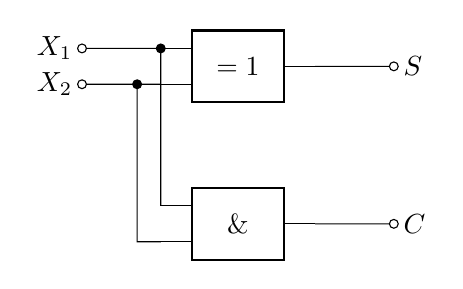
\begin{tikzpicture}
			\ctikzset{logic ports=european,tripoles/european not symbol=ieee circle}
			\draw
			(0,0) node[xor port] (xor1) {}
			(0,-2) node[and port] (and1) {}
			(xor1.out) to[short , -o] ++(1,0) node[right]{\(S\)}
			(and1.out) to[short , -o] ++(1,0) node[right]{\(C\)}
			(xor1.in 1) to[short, -o] ++(-1,0) coordinate(x1) node[left]{\(X_1\)}
			(xor1.in 1) to[short, *-] (and1.in 1)
			(xor1.in 2) -- ++(-0.3,0) coordinate(j1)
			(j1) to[short, *-] (j1 |- and1.in 2) -- (and1.in 2)
			(j1) to[short, -o] (x1 |- xor1.in 2) node[left]{\(X_2\)}
			;
		\end{tikzpicture}
		\caption{Gate Level Description of Half Adder}
		\label{HA_GateLevel}
	\end{center}
\end{figure}

is a combinational logic circuit shown in Figure.(\ref{HA_GateLevel}) that takes two binary inputs and produces two binary outputs: sum and carry.

\begin{eqnarray}
	\mathop{\mathrm{HA}}:(x_1,x_2)\mapsto(Q,C) :=
	\begin{cases}
		Q & =\mathop{\mathrm{xor}}(x_1,x_2) \\
		C & =\mathop{\mathrm{and}}(x_1,x_2)
	\end{cases}
\end{eqnarray}

The main limitation of the half adder is that it cannot handle carry inputs and therefore can only be used for 1-bit addition.

A \textit{full adder} is an extension of the half adder that accepts three binary inputs: two additions and a rounding input, and produces two binary outputs: sum and carry. Full adders can be connected in series to achieve binary addition of any number of bits.

\begin{figure}[htpb]
	\begin{center}
		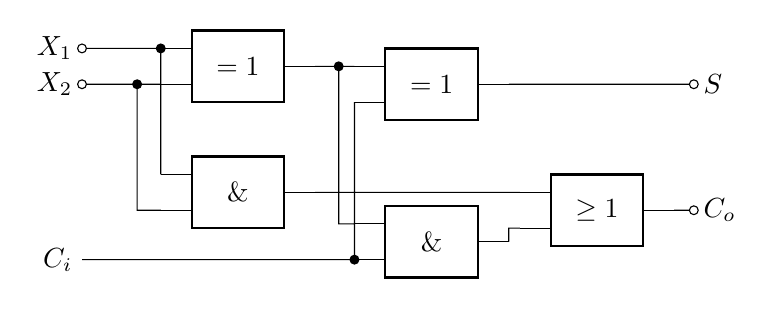
\begin{tikzpicture}
			\ctikzset{logic ports=european,tripoles/european not symbol=ieee circle}
			\draw
			(0,0) node[xor port] (xor1) {}
			(0,-1.6) node[and port] (and1) {}
			(xor1.out) ++(0.5,0) node[xor port, anchor=in 1] (xor2) {}
			(xor1.out) ++(0.5,-2) node[and port, anchor=in 1] (and2) {}
			(and1.out) ++(2.6,0) node[or port, anchor=in 1] (or1) {}
			(xor1.in 1) to[short, -o] ++(-1,0) coordinate(x1) node[left]{\(X_1\)}
			(xor1.in 1) to[short, *-] (and1.in 1)
			(xor1.in 2) -- ++(-0.3,0) coordinate(j1)
			(j1) to[short, *-] (j1 |- and1.in 2) -- (and1.in 2)
			(j1) to[short, -o] (x1 |- xor1.in 2) node[left]{\(X_2\)}
			(x1 |- and2.in 2) coordinate(ci) node[left]{\(C_i\)}
			(xor1.out) -- ++(0.3,0) coordinate(j2) to[short, *-] (xor2.in 1)
			(j2) |- (and2.in 1)
			(ci) -| (and2.in 2)
			(and2.in 2) to[short, *-] (xor2.in 2)
			(and1.out) |- (or1.in 1)
			(and2.out) |- (or1.in 2)
			(or1.out) to[short, -o] ++(0.25,0) coordinate(co) node[right]{\(C_o\)}
			(xor2.out) to[short, -o] (co |- xor2.out) node[right]{\(S\)}
			;
		\end{tikzpicture}
		\caption{Gate Level Description of Full Adder}
		\label{FA_GateLevel}
	\end{center}
\end{figure}

Implementation of full adder can be derived directly from 3-digit addition, where the final carry output is toggled if any of \(X_1+X_2\) or \(C_i+Q_1\) produces a carry:

\begin{eqnarray}
	(q_1,c_1)&=\mathop{\mathrm{HA}}(x_1,x_2) \\
	(q_2,c_2)&=\mathop{\mathrm{HA}}(q_1,c_i) \\
	c_o &= \mathop{\mathrm{or}}(c_1,c_2)
\end{eqnarray}

Therefore the gate-level circuit of the full adder can be easily captured, as shown of Figure.(\ref{FA_GateLevel})

\section{Verilog Modeling}

There are two levels of HDL modeling for full adder, one for gate level description and one for behavioral level description.

\subsection{Gate-Level Implementation}

\lstinputlisting[caption={Gate Level Modeling of Full Adder in Verilog}, language=verilog, style=verilog, label=glm_fa, linewidth=0.92\linewidth]{../../lab2/lab2.srcs/sources_1/new/full_adder_g.v}

For the gate level modeling, the DNF (OR-AND) of the output ports are required:

\begin{eqnarray}
	\begin{aligned}
		Q_2              & =HA(HA(x_1,x_2)[0],c_i)[0]                                           \\
		                 & =\mathop{\mathrm{xor}}(\mathop{\mathrm{xor}}(x_1,x_2),c_i)           \\
		                 & = \overline{AB} C+\overline{A} B \overline{C} + A \overline{BC} +ABC \\
		C_{\mathrm{out}} & =AB+BC+AC
	\end{aligned}
\end{eqnarray}

Therefore, the Verilog code is pretty straight forward, as the Code.(\ref{glm_fa}). For the Vivado elaboration and synthesis process, the logic functions are expanded to its DNF, meaning only AND/OR/NOT gates remains in the elaborated schematic:

\begin{figure}[htpb]
	\begin{center}
		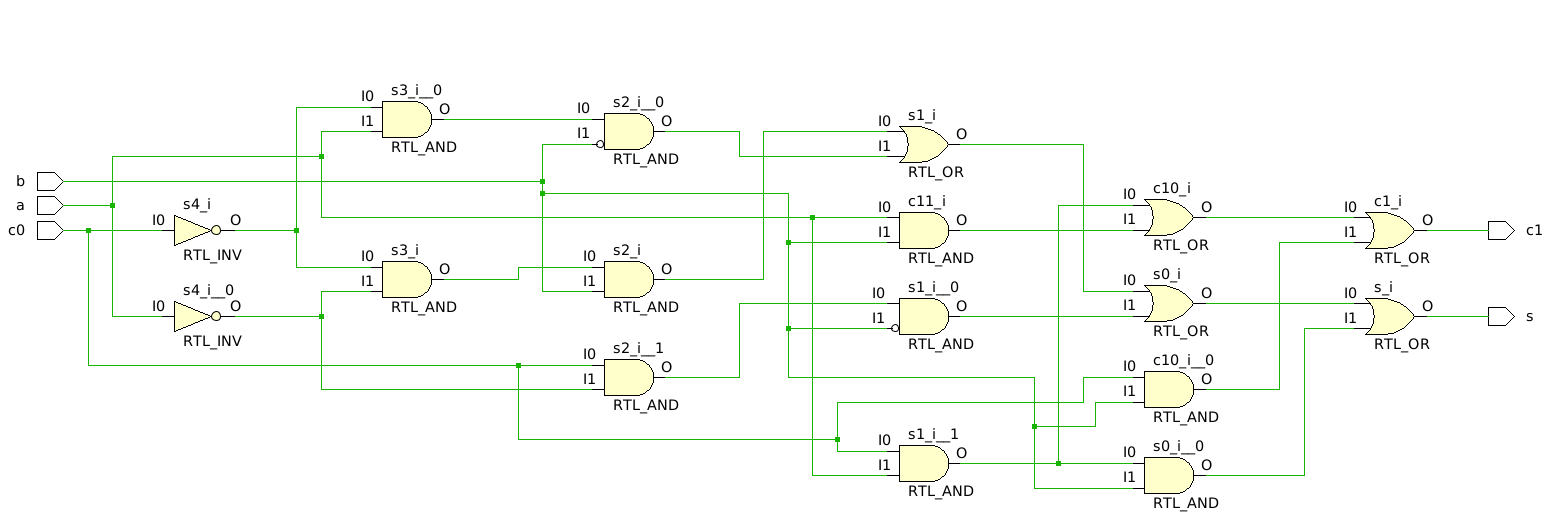
\includegraphics[width=0.97\linewidth]{report_lab2.assets/20240307171752.png}
		\caption{Elaborated Gate Level Description}
		\label{elaborated_gl_sch}
	\end{center}
\end{figure}

\subsection{LUT Implementation}

\lstinputlisting[caption={Gate Level Modeling of Full Adder in Verilog}, language=verilog, style=verilog, label=glm_fa, linewidth=0.92\linewidth]{../../lab2/lab2.srcs/sources_1/new/full_adder_lut.v}

The combine logic functions are implemented by LUT(Look-Up Table)s inside the FPGA components in real world, while the half adder is a common LUT element inside the CLBs. By simply configuring the switchable connections between the CLBs and the controlling MUXs inside the CLBs, a cascaded design can be easily obtained.

\begin{figure}[htpb]
	\begin{center}
		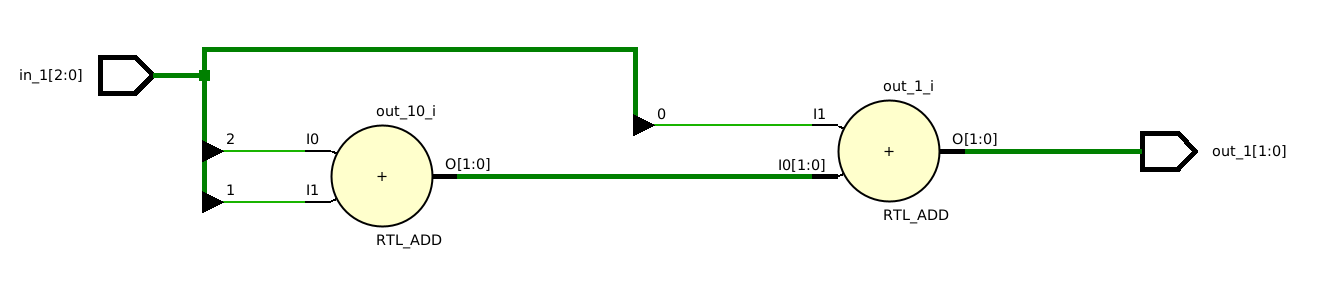
\includegraphics[width=0.97\linewidth]{report_lab2.assets/20240307172354.png}
		\caption{Elaborated RTL Level Description}
		\label{elaborated_lut_level_sch}
	\end{center}
\end{figure}

\subsection{Synthesized Implementation}

\begin{figure}[htpb]
	\begin{center}
		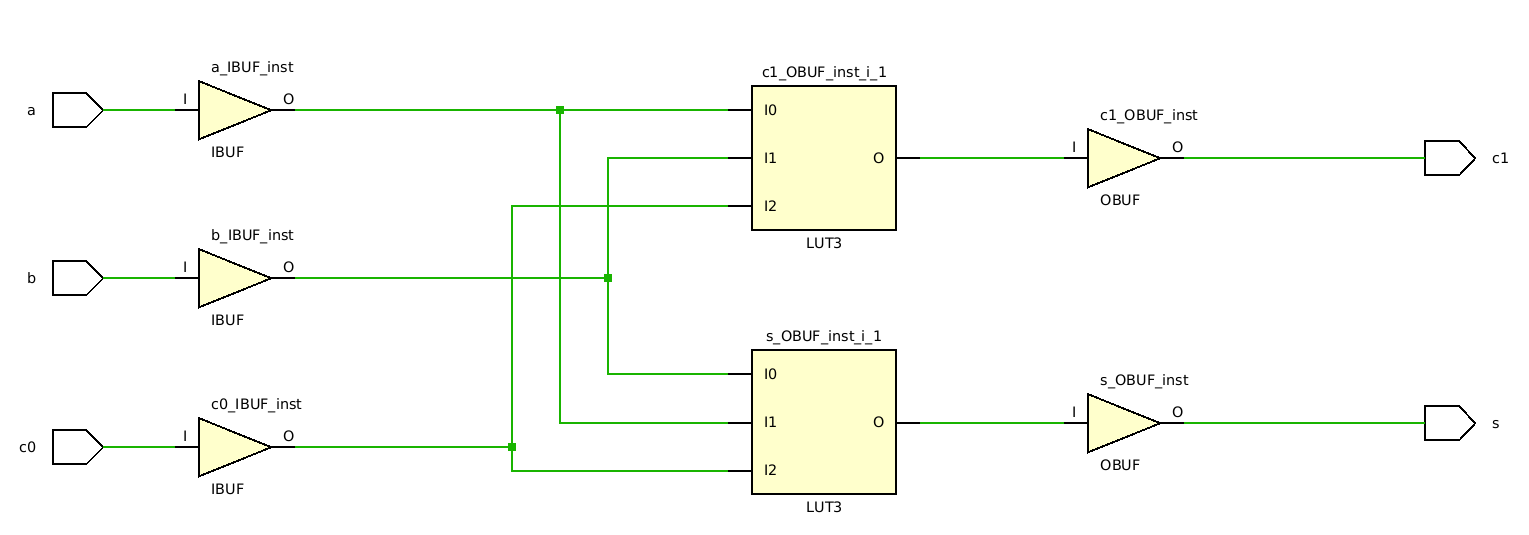
\includegraphics[width=0.97\linewidth]{report_lab2.assets/20240307172835.png}
		\caption{Synthesized Design}
		\label{FA_synth}
	\end{center}
\end{figure}

Either the gate level design (\ref{elaborated_gl_sch}) or the RTL level design (\ref{elaborated_lut_level_sch}) are synthesized into the same schematic (\ref{FA_synth}) after the synthesis and implementation process, since the FPGA device only provide configurable LUT as the measure to combinational logic inside the CLB.

In the synthesized schematic (\ref{FA_synth}), the two LUT cells are combinational logic functions of \(S=\mathop{\mathrm{LUT_1}}(X_0,X_1,C_i)\) and \(C_o=\mathop{\mathrm{LUT_2}}(X_0,X_1,C_i)\) respectively.

\section{Simulation}

\begin{table}
	\begin{center}
		\begin{tabular}[htb]{ccccccc}
			\toprule
			\(X_1\) & \(X_0\) & \(C_i\) & \(\mathop{\mathrm{dec}}(in[2:0])\) & \(C_o\) & \(S\) & \(\mathop{\mathrm{dec}}(out[1:0])\) \\
			\midrule
			0       & 0       & 0       & 0                                  & 0       & 0     & 0                                   \\
			0       & 0       & 1       & 1                                  & 0       & 1     & 1                                   \\
			0       & 1       & 0       & 2                                  & 0       & 1     & 1                                   \\
			0       & 1       & 1       & 3                                  & 1       & 0     & 2                                   \\
			1       & 0       & 0       & 4                                  & 0       & 1     & 1                                   \\
			1       & 0       & 1       & 5                                  & 1       & 0     & 2                                   \\
			1       & 1       & 0       & 6                                  & 1       & 0     & 2                                   \\
			1       & 1       & 1       & 7                                  & 1       & 1     & 3                                   \\
			\bottomrule
		\end{tabular}
		\caption{Truth Table of Full Adder}
		\label{tt_fa}
	\end{center}
\end{table}

The truth table of the full adder is Table.(\ref{tt_fa}). For the design using gate-level description, simulation result is shown in the waveform figure corresponding to each stage:

\begin{itemize}
	\item Figure.\ref{sim_result}\subref{sim_behv}: \textbf{behavioral} simulation after \textbf{elaboration}
	\item Figure.\ref{sim_result}\subref{sim_synth}: \textbf{timing} simulation after \textbf{synthesis}
	\item Figure.\ref{sim_result}\subref{sim_impl}: \textbf{timing} simulation after \textbf{implementation}
\end{itemize}

\begin{figure}[htpb]
	\begin{center}
		\subfloat[Behavioral Simulation]{\label{sim_behv}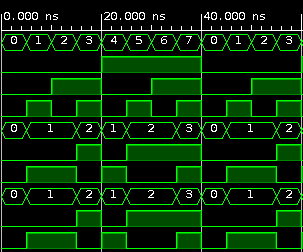
\includegraphics[width=0.45\columnwidth]{report_lab2.assets/20240307184341.png}}\hspace{0.05\columnwidth}
		\subfloat[Timing after Synthesis]{\label{sim_synth}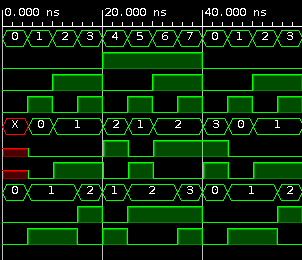
\includegraphics[width=0.45\columnwidth]{report_lab2.assets/20240307184023.png}}\\
		\subfloat[Timing after Implementation]{\label{sim_impl}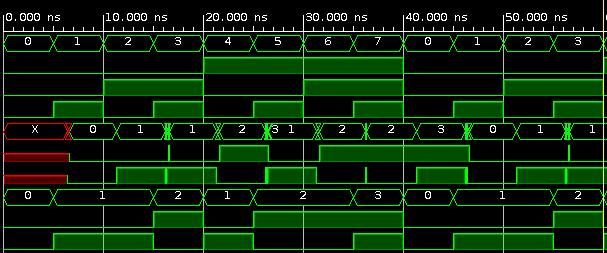
\includegraphics[width=0.97\columnwidth]{report_lab2.assets/20240307184637.png}}
		\caption{Simulation Results}
		\label{sim_result}
	\end{center}
\end{figure}

Additionally, the timing simulation result of the design using RTL block-level description after implementation is also provided in Figure.(\ref{sim_impl_rtlblk}), since the only difference between the block-level version and the gate-level version is the routing after implementation.

\begin{figure}[htpb]
	\begin{center}
		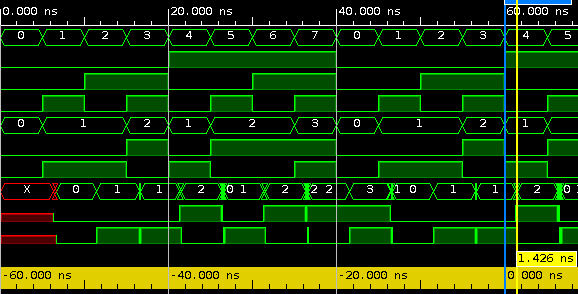
\includegraphics[width=0.97\linewidth]{report_lab2.assets/20240307190951.png}
		\caption{Timing Simulation of RTL Block-level Design}
		\label{sim_impl_rtlblk}
	\end{center}
\end{figure}

Vivado only accepts one single top file in one synthesis/implementation batch, resulting that only one module can be accurately simulated at implemented level, while the others remains behavioral level. In the following discussions, the behavioral level trail are considered as a marking for comparison.

\subsection{Consistency}

Comparing result Figure.\ref{sim_result}\subref{sim_behv} from both gate-level and RTL-level designs with the truth table Table.\ref{tt_fa}, it is easy to identify that the behavioral simulation result is consistent with the truth table. Therefore the consistency is verified.

However, there exists one difference between the behavioral simulation result and the waveforms shown in lecture notes, that the result from Vivado simlulation returns its output immediately after the initial Hi-Z undeterministric state, while the result in lecture notes shows that there is additional delay from the end of Hi-Z state to the first sensible output. The reason to this phenomenon can be the optimizations done by Vivado elaborator.

\subsection{Delay}

Compare the other 2 simulation results with the behavioral simulation result, the initial undetermined state is conspicuous since it is marked in eye-catching red highlights, while there is no undetermined regions or time domain offsets in behavioral simulation result suggesting the existence of delays.

Additionally, the delay of gate-level design after implementation is slightly higher than that of an RTL-level design, by comparing the time the system remains undetermined state. The reason to this phenomenon can be the different path length between CLBs used in the different design, and the RTL-level design using half adder suggests the elaborator and synthesizer to route a path with lower distance.

\subsection{Jitters}

Contrast the position of the jitter in the output waveform with the edge of the input waveform on the time axis, the moments when the output waveform has a jitter are easily found to correspond to the moments when both the rising and falling edges of the multiple input waveforms are present plus a gate delay.

\begin{figure}[htpb]
	\begin{center}
		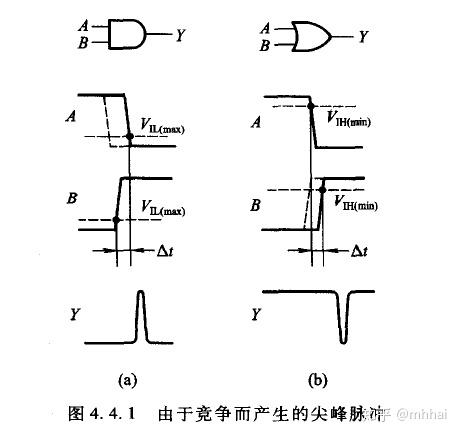
\includegraphics[width=0.75\linewidth]{report_lab2.assets/20240308154213.png}
		\caption{Explanation of Race Conditions}
		\label{race_cond_explain}
	\end{center}
\end{figure}

By referencing the schematic of the synthesized design, there only exists one single element between the multiple inputs with race conditions and both of the output port, thus the delay between the emergence of race condition \ref{race_cond_explain} and the spikes in output is the unit delay of one single LUT element.

\section*{\textbf{Appendix.} Testbench}

\lstinputlisting[caption={Testbench}, language=verilog, style=verilog, label=glm_fa, linewidth=0.92\linewidth]{../../lab2/lab2.srcs/sim_1/new/FA_tb.v}

\end{document}